\subsection{Plastic plate - Cam-Clay plasticity (2D)}
\label{sec:ccup}

\subsubsection*{Problem definition}

This example is generally applied to verify a critical state plastic
mode, i.e. Cam-Clay model. We consider a quarter of the cylindrical
sample of 5cm in diameter and 10cm in length.

\subsubsection*{Initial and Boundary conditions}

The bottom surface is roller supported.
A vertical down displacement is prescribed to make an axial strain of 50\%. The movement in the radial
direction on the top surface is allowed. The cylindrical  surface is traction free.

\subsubsection*{Material properties}

Table \ref{tab:m_cc_s} shows the material parameters.
 \begin{table}[H]
\begin{tabular}{lrl}
\hline\noalign{\smallskip}
  \hline
 Meaning & Value & Unit \\
  \hline
 Poisson ratio & $0.3$ & ---\\
 Slope of the critical state line & $1.2$ & ---\\
 Virgin compression index & $0.2$ & ---\\
 swelling/recompression index & $0.02$ & ---\\
 Initial preconsolidation pressure & $60.0$ & $--$\\
 Initial void ratio & $1.5$ & $--$\\
 \hline\hline
\end{tabular}
\caption{Solid material properties} %\footnotesize
\label{tab:m_cc_s}
\end{table}

\subsubsection*{Results}

The problem is axisymmetrical. A relationship between von Mises type stress, the second stress invariant, and the axial strain is illustrated in Fig. \ref{fig:m_cc_s_r}. The results agrees with what given in \cite{SheSloYu00}.

\begin{figure}[H]
  \begin{center}
    \includegraphics[scale=0.3]{M/cc_s_s_e.eps}
  \end{center}
  \caption{Axial strain vs von Mises type stress }
  \label{fig:m_cc_s_r}
\end{figure}

\subsubsection*{Benchmark deposit}

\begin{tabular}{|l|l|l|}
  \hline
  Benchmark & Problem type & Path in benchmark deposit \\
  \hline
 \emph{m\_cc\_quad\_s}\&  \emph{m\_cc\_tri\_s}& M & benchmarks\verb \M\ \\
  \hline
\end{tabular}

